\chapter{Mechanical Design}

This chapter covers the mechanical design of the hydrogel bioprinter using the standard engineering design process that involves the identification of both stakeholder and engineering requirements, the application of a morphological analysis, and the final design. The 3D printer system must fulfil two primary functions:
\begin{itemize}
    \item Extrude hydrogel (specifically GelMA).
    \item Position the extruder in 3D space.
\end{itemize}


\section{Stakeholder Requirements}

The development of the hydrogel bioprinter is performed in accordance to the purpose of its use and the needs of its stakeholders. The 3D printer is being developed in order to serve as a research tool for SU's Physiology Department, in which it will be used as an apparatus for characterising bioinks and creating hydrogel scaffolds (acellular or seeded with cells) to model and simulate cellular growth in biomedical research. The stakeholders whose needs guide the design of the system include the physiology researchers (end-users), the engineering student developing the printer, regulatory authorities that require compliance with health and safety standards as well the strict sanitary standards that need to be met in biomedical research, and Stellenbosch University by which the project is funded. While not strictly a mandority requirement, the system should also meet the needs of any future designer that is tasked with upgrading the system or adding additional functionalities to the printer. The requirements that the system must/should meet in order to fulfil the needs of these stakeholders are tabulated below in Table~\ref{tab:stakeholder_requirements}.

\small
\begin{longtable}{|c|m{2.2cm}|m{7.3cm}|c|}
\caption{Stakeholder Requirements}
\label{tab:stakeholder_requirements} \\
\hline
\textbf{No.} & \textbf{Stakeholder} & \textbf{Description} & \textbf{Priority} \\
\hline
SR1 & Researchers (End-users) & The system must be able to extrude hydrogel to create 3D hydrogel scaffolds & must-have \\
\hline
SR2 & Designer (Engineer) & The printer should be able to precisely, accurately, and smoothly adjust the position of the extruder in 3D space\textsuperscript{1} & must-have \\
\hline
SR3 & Designer (Engineer) & The extruder must be able to accurately and precisely control the flow rate of hydrogel being extruded\textsuperscript{1} & must-have \\
\hline
SR4 & Researchers (End-users) & The system should support the real-time gelation of the bioink during print tasks\textsuperscript{2} & must-have \\
\hline
SR5 & Researchers (End-users) & The bioprinter should support multiple types of hydrogel\textsuperscript{3} & must-have \\
\hline
SR6 & Researchers (End-users) & The printer should have a repeatable performance for unique set of parameters\textsuperscript{1} & must-have \\
\hline
SR7 & Researchers (End-users) & The printer must allow for tunable parameters\textsuperscript{3} & must-have \\
\hline
SR8 & Researchers (End-users) & The system should be user-friendly and simple to operate\textsuperscript{4} & must-have \\
\hline
SR9 & Biosafety Authorities & The extruder must be sterilisable and come with a documented cleaning procedure\textsuperscript{5} & must-have \\
\hline
SR10 & Health and Safety Authorities & The system should be safe to handle with minimized risks to the health and safety of its users & must-have \\
\hline
SR11 & SU's finance department & The printing system as a whole should be affordable and meet budget requirements\textsuperscript{6} & must-have \\
\hline
SR12 & Researchers (End-users) & The system must include a documented experimental procedure to calibrate the bioprinter to perform optimised prints of desired bioinks\textsuperscript{3} & must-have \\
\hline
SR13 & Researchers (End-users) & The system should be able to transmit real time experimental data\textsuperscript{3} & optional \\
\hline
SR14 & Designer (Engineer) & The printer should include feedback control for precise operation & optional \\
\hline
SR15 & Future Designers & The printer should be modular and allow for future upgrades\textsuperscript{7} & optional \\
\hline
\end{longtable}
\noindent\textsuperscript{1} The calibrated printer should perform prints that accurately match the desired print tasks and do not vary across iterations with a specific set of printer settings.

\noindent\textsuperscript{2} This means that the printer should support the solidification of the gel during print operations to ensure the structural integrity of printed scaffolds.

\noindent\textsuperscript{3} These requirements are needed for the system to fulfil its role in serving as a tool for characterising bioinks and calibrating the printer to perform optimised prints.

\noindent\textsuperscript{4} The end-users are not engineers and the printer should therefore be simple to operate by researchers without technical knowledge of mechatronic systems.

\noindent\textsuperscript{5} The printer must be cleaned and sterilised throughout its lifetime to ensure bioink viability and compliance with health standards.

\noindent\textsuperscript{6} This excludes resources that will be sourced from within the University of Stellenbosch.

\noindent\textsuperscript{7} Future upgrades may include adding a user interface or developing an additional extruder for dual extrusion.

\section{Engineering Requirements}
Although the needs of the stakeholders have been identified, they must be transformed into engineering requirements that define how the system will satisfy these needs. They functional and performance requirements.

Both Tables~\ref{tab:func_requirements} and~\ref{tab:nonfunc_requirements} below, shows the bioprinter's engineering requirements (both functional and non-functional).

\small
\begin{longtable}{|c|m{8.1cm}|l|}
\caption{Functional Requirements} 
\label{tab:func_requirements} \\
\hline
\textbf{No.} & \textbf{Description} & \textbf{Related SR} \\
\hline
\endfirsthead
\hline
\textbf{No.} & \textbf{Description} & \textbf{Related SR} \\
\hline
\endhead
FR1 & The printer must be able to move the extruder along three axes (relative to a printing platform) with precise positional control. & SR2, SR6 \\
\hline
FR2 & The system must extrude hydrogel at a desired and controlled flow rate. & SR1, SR3 \\
\hline
FR3 & The printer must have the ability to include UV curing with adjustable intensity that operates during extrusion. & SR4 \\
\hline
FR4 & The printer must include the ability to adjust bioink fluid properties by bed and nozzle temperature control. & SR7, SR9 \\
\hline
FR5 & The printer firmware must allow for the adjustment of printer parameters such as nozzle and bed temperature, extrusion speed, and travel speed. & SR7 \\
\hline
FR6 & The system should be able to transmit sensory feedback for system control and to capture real-time data during the printer's calibration. & SR13, SR14 \\
\hline
FR7 & The printer must include feedback control for precise operation. & SR14 \\
\hline
\end{longtable}

\small
\begin{longtable}{|c|m{8.1cm}|l|}
\caption{Non-Functional Requirements (Constraints)}
\label{tab:nonfunc_requirements} \\
\hline
\textbf{No.} & \textbf{Description} & \textbf{Related SR} \\
\endfirsthead
\hline
\hline
\textbf{No.} & \textbf{Description} & \textbf{Related SR} \\
\hline
\endhead
NFR1 & The extruder/bioink fluid path must be removable and capable of being cleaned and sterilised. & SR9 \\
\hline
NFR2 & The printer should be modular to support future upgrades. & SR15 \\
\hline
NFR3 & The printer must be affordable and within the allocated SU final year project budget. & SR11 \\
\hline
NFR4 & The design, development, and use of the bioprinter must comply with Stellenbosch University's health and safety regulations. & SR10, SR11 \\
\hline
NFR5 & The system should be user-friendly and simple to operate. & SR8 \\
\hline
NFR6 & The bioprinter should support multiple types of hydrogel. & SR5 \\
\hline
NFR7 & The system must include a documented procedures to calibrate the bioprinter to desired hydrogels and clean after use & SR9, SR12 \\
\hline
\end{longtable}


The performance requirements, documented in Table~\ref{tab:performance_requirements}, quantify how well the system must meet its functional requirements. The target levels for each performance requirement was chosen to match the performance capabilities of the current state of the art for bioprinters (such as the Bio X) as far as reasonably possible.

\small
\begin{longtable}{|c|m{5.5cm}|c|c|c|m{1.5cm}|}
\caption{Performance Requirements}
\label{tab:performance_requirements} \\
\hline
\textbf{No.} & \textbf{Description} & \textbf{Target} & \textbf{Range} & \textbf{Unit} & \textbf{Related FR} \\
\hline
\endfirsthead
\hline
\textbf{No.} & \textbf{Description} & \textbf{Target} & \textbf{Range} & \textbf{Unit} & \textbf{Related FR} \\
\hline
\endhead
PR1 & Extrusion speed & 5 & 3 - 15 & mm/s & FR2 \\
\hline
PR2 & Positional accuracy along XY axes & 100 & 50 - 500 & $\mu$m
 & FR1 \\
\hline
PR3 & Positional accuracy along Z axis & 50 & 25 - 100 & $\mu$m
 & FR1 \\
\hline
PR4 & Maximum travel speed along XY axes & 50 & 30 - 70 & mm/s & FR1 \\
\hline
PR5 & Maximum travel speed along Z axis & 30 & 20 - 50 & mm/s & FR1 \\
\hline
PR6 & Minimum bed temperature\textsuperscript{1} & 4 & < 20 & $^{\circ}$C & FR4 \\
\hline
PR7 & Maximum nozzle temperature\textsuperscript{2} & 85 & 80 < & $^{\circ}$C & FR4 \\
\hline
PR8 & Nozzle temperature control tolerance & $\pm$ 1 & $\pm$ 0.5 – 2 & $^{\circ}$C & FR4 \\
\hline
PR9 & Extrusion force control setpoint tolerance & $\pm$ 5 & $\pm$ 2 – 10 & \% & FR2, FR7 \\
\hline
\end{longtable}
\noindent\textsuperscript{1} This matches the Bio X's minimum bed temperature capability of 4 $^{\circ}C$ \citep{biox_brochure}.

\noindent\textsuperscript{2} The target matches the maximum capability of the Bio X's pneumatic print heads \citep{biox_brochure}.

\section{Extruder Design}
The rest of this chapter will cover the design of each of the bioprinter’s subsystems, using a concept generation and selection process, followed by the final design. Since the system’s two primary functions are to extrude gel and position the extrusion nozzle in 3D space, these functions serve as the basis for dividing the system into its respective subsystems (extruder and gantry). This section focuses on the extruder design, starting with the development of generated concepts.

\subsection{Concept Generation}
\subsubsection*{Concept 1}
The first concept, shown in Figure~\ref{fig:pumpConcept}, illustrates a pump-based extruder design in which a peristaltic pump is used to drive the continuous flow of non-gelled bioink from a fluid reservoir. The reservoir could take the form of either a permanent or intermediate temporary storage for the gel ink (configured to create the correct handling conditions) and not necessarily in the beaker-shaped form shown in the figure.

\begin{figure}[H]
    \centering
    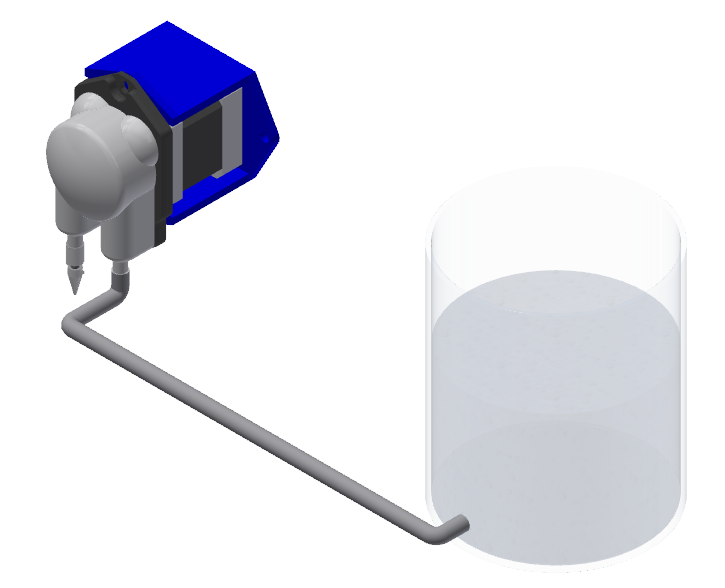
\includegraphics[scale=0.35]{figs/PumpConcept.png}
    \caption{Concept 1 Pump-Based Extruder Design}
    \label{fig:pumpConcept}
\end{figure}

\subsubsection*{Concept 2}
Figure~\ref{fig:syringeConcept1} shows the second concept that consists of an assembly of 3D printed parts, in which a stepper motor drives two lead screws (through a system of printed gears) to push a plunger further into a store-bought syringe. The pre-existing syringe is easily removable by either unbolting the flanged tube in which the syringe sits or by sliding the syringe out vertically when the platform that pushes the plunger is in its uppermost position. The inclusion of gears is used to allow the plunger to be driven with a greater force magnitude for extruding high-viscosity gels through small-diameter nozzles.

\begin{figure}[H]
    \centering
    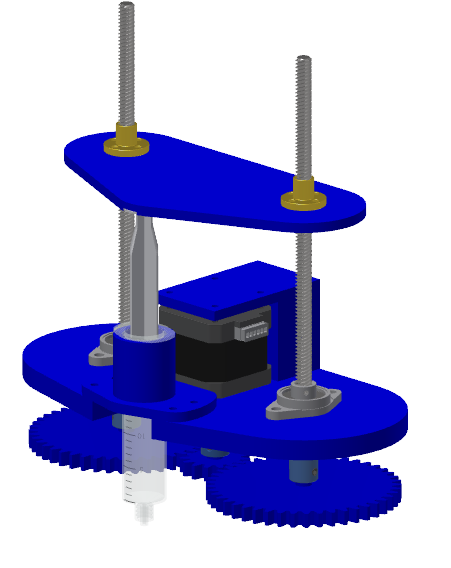
\includegraphics[scale=0.7]{figs/SyringeConcept1.png}
    \caption{Concept 2 Syringe-Based Extruder Design}
    \label{fig:syringeConcept1}
\end{figure}

\subsubsection*{Concept 3}
The final concept, in Figure~\ref{fig:syringeConcept2}, shows another syringe-based extruder like the second concept. This concept deviates from the previous one in a few ways, including its syringe, material composition, and actuation style. This concept uses a custom-made aluminium syringe with a PVC plunger and threaded nozzle to accept screw-in component additions (for added modularity). This concept is also made up of additional machined aluminium platforms. The extruder uses a GT2 belt-and-pulley drive-train to increase the force of the lead screw on the plunger and also uses a shaft to guide the plunger-driving platform.
\begin{figure}[H]
    \centering
    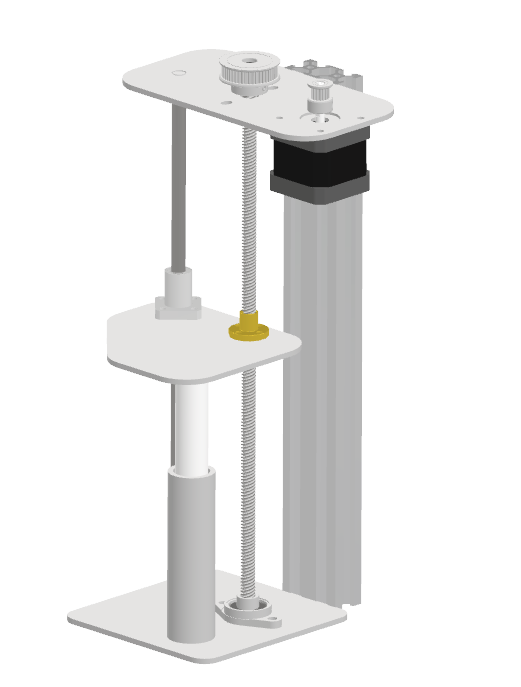
\includegraphics[scale=0.65]{figs/SyringeConcept3.png}
    \caption{Concept 3 Custom Syringe-Based Extruder Design}
    \label{fig:syringeConcept2}
\end{figure}

\subsection{Concept Evaluation and Selection}
To objectively evaluate the three generated concepts and identify the one that best satisfies the project’s stakeholder requirements, a Pugh chart was developed. This method compares each concept against multiple weighted criteria, each derived from a specific stakeholder requirement. Concept 2 was selected as the reference datum, and the other concepts were rated relative to it on a scale from –2 to +2, with positive values indicating favourable performance and negative values indicating less favourable performance. Table~\ref{tab:pugh1} presents the results of the Pugh chart evaluation.

\begin{sidewaystable}[p]
\centering
\caption{Concept Evaluation (Pugh Chart)}
\label{tab:pugh1}
\renewcommand{\arraystretch}{1.2}
\setlength{\tabcolsep}{3.5pt}

\begin{tabular}{|>{\centering\arraybackslash}p{35mm}|
                >{\centering\arraybackslash}p{15mm}|
                >{\centering\arraybackslash}p{15mm}|
                >{\raggedright\arraybackslash}p{35mm}|
                >{\centering\arraybackslash}p{15mm}|
                >{\raggedright\arraybackslash}p{35mm}|
                >{\centering\arraybackslash}p{15mm}|
                >{\raggedright\arraybackslash}p{35mm}|}
\hline
\multicolumn{2}{|c|}{\textbf{Criterion}} &
\multicolumn{2}{c|}{\textbf{Concept 1}} &
\multicolumn{2}{c|}{\textbf{Concept 2}} &
\multicolumn{2}{c|}{\textbf{Concept 3}} \\
\hline
\textbf{Description} & \textbf{Weight} &
\textbf{Rating} & \textbf{Motivation} &
\textbf{Datum} & \textbf{Motivation} &
\textbf{Rating} & \textbf{Motivation} \\
\hline
Maximum flow rate (SR1) & 0.07 & +2 & Higher throughput & 0 & Limited by lead screw & 0 & Limited by lead screw \\\hline
Maximum extrusion force (SR1) & 0.13 & -2 & Pressure drop across longer fluid path & 0 & Limited by the buckling of the plastic plunger & +2 & High due to lead screw, drive-train and aluminium syringe \\\hline
Ink storage volume (SR1) & 0.05 & +2 & Large reservoir and continuous pump action & 0 & Limited by syringe volume & 0 & Limited by syringe volume \\\hline
Flow rate accuracy (SR3) & 0.19 & -1 & Inaccurate at low speeds & 0 & Accurate due to lead screw and gear reduction & +1 & Accurate due to lead screw and drive-train \\\hline
Support multiple hydrogels (SR5) & 0.13 & -2 & Tubing limits viscous gels & 0 & Moderate viscosity acceptable & +1 & Metal path can handle highly viscous inks \\\hline
Repeatable performance (SR6) & 0.15 & -1 & Tube ageing & 0 & Variable backlash from printed gears & +2 & Low backlash from tensioning \\\hline
Sterilisability and cleanability (SR9) & 0.13 & -2 & Hard to clean long path & 0 & Removable syringe and straight path & 0 & Removable syringe and straight path \\\hline
Affordability (SR11) & 0.15 & -2 & Requires a peristaltic pump & 0 & 3D printing and standard parts & -1 & Standard parts and machined metal \\\hline
\hline
\multicolumn{2}{|l|}{\textbf{Sum of plus ratings}} &
\multicolumn{2}{c|}{4} &
\multicolumn{2}{c|}{0} &
\multicolumn{2}{c|}{6} \\\hline

\multicolumn{2}{|l|}{\textbf{Sum of minus ratings}} &
\multicolumn{2}{c|}{-10} &
\multicolumn{2}{c|}{0} &
\multicolumn{2}{c|}{-1} \\\hline

\multicolumn{2}{|l|}{\textbf{Overall total}} &
\multicolumn{2}{c|}{-6} &
\multicolumn{2}{c|}{0} &
\multicolumn{2}{c|}{5} \\\hline

\multicolumn{2}{|l|}{\textbf{Weighted total}} &
\multicolumn{2}{c|}{-1.18} &
\multicolumn{2}{c|}{0} &
\multicolumn{2}{c|}{0.73} \\\hline

\end{tabular}
\end{sidewaystable}

\FloatBarrier

The Pugh chart indicates that Concept 3 provides the most favourable balance across the weighted criteria. Its high flow rate accuracy is achieved through the use of a lead screw and drive-train, which also enables it to deliver the greatest extrusion forces. Although less affordable than a 3D-printed design, the use of machined metal components ensures these high extrusion forces can be produced without compromising structural integrity. Together, these factors enable the extruder to handle highly viscous gels with repeatable performance while maintaining sterilisability.

\subsection{Final Extruder Design}
With Concept 3 selected as the most suitable option, the concept is refined into a final extruder design that is ready for assembly. In this subsection, the extruder is specified in detail, with calculations provided to quantify its design requirements (stepper torque, pulley ratios, and plunger dimensions) and to determine its theoretical performance characteristics such as flow rate resolution. These demonstrate that the final design meets the stakeholder requirements.
\subsubsection*{Extrusion Force Calculations}
To calculate the needed stepper torque and pulley ratio, it is first necessary to describe the system characteristics and requirements. The syringe should hold roughly \SI{25}{mL} and therefore has an internal diameter of \SI{20}{mm} and a length of \SI{80}{mm}. The nozzle’s threaded shank provides attachment for an E3D hot-end assembly that can accommodate different nozzle diameters. To be conservative and to allow printing with high accuracy, the design assumes the ability to extrude through a minimum nozzle diameter of \SI{0.2}{mm} with an approximate length of \SI{20}{mm}. To ensure compatibility with multiple hydrogels, the extruder is specified to handle gels with a maximum viscosity of $10~\si{\pascal\second}$.

These assumptions are restated in Appendix~A.1, which shows, using Poiseuille’s Law, that extrusion under these edge-case conditions requires the plunger to deliver a maximum pressure of $900~\si{\kilo\pascal}$. The calculations further indicate that, to achieve this pressure over the cylinder’s cross-sectional area, the lead screw must apply approximately \SI{300}{N} of force on the plunger. This corresponds to a torque requirement of $0.638~\text{N}\cdot\text{m}$ for the TR8$\times$8 lead screw. To achieve this, a NEMA17 stepper motor with a maximum holding torque of $0.28~\text{N}\cdot\text{m}$ is used in combination with a 3:1 GT2 pulley reduction (48T:16T), increasing the maximum torque at the lead screw to $0.84~\text{N}\cdot\text{m}$. The conservative assumption of assuming a nozzle length of 20 mm and a maximum viscosity of $10~\si{\pascal\second}$ serves as a safety factor that provides protection against worst-case scenarios such as nozzle clogging.


\subsubsection*{Flow Rate Resolution}
The minimum flow rate resolution without microstepping can be determined based on the relationship between the angle of the motor shaft, lead screw pitch, and the cross-sectional area inside the syringe. Since the system uses a pulley ratio (PR) of 3:1, the lead is \SI{8}{mm}, and the motor is adjusted by $1.8^{\circ}$ per full step, the positional accuracy with which the plunger can move is:

\begin{align*}
\Delta x_{\text{Full Step}} &= \frac{\text{Lead}}{\text{PR}} \times \frac{\theta_{\text{Full Step}}}{360^{\circ}} \\
&=\frac{8.00}{3}\times \frac{1.8^\circ}{360^\circ} \\
&= 0.0133~\text{mm}/\text{step}
\end{align*}

\noindent To convert this to a volumetric resolution, this value must be multiplied by the cross-sectional area of the syringe through which the plunger slides:
$$\Delta V_\text{Full Step} =\pi \left(10 \times 10^{-3}\right)^2 (1.33 \times 10^{-5})=4.19\times10^{-9} \,\,\text{m}^3/\text{step} =\boxed{4.19~\mu\text{L}/\text{step}} 
$$
Therefore, the extruder has a minimum theoretical extrusion resolution of $4.19~\mu\text{L}$ for a full step that drives the stepper. This resolution can be further refined through microstepping.

\subsubsection*{Buckling Analysis}
The syringe plunger is made of PVC, and the minimum diameter of the plunger stem must be determined to avoid buckling under the extrusion-force edge case of \SI{300}{N}. According to \cite{callister2018materials}, the modulus of elasticity of PVC ranges from \SI{2.41}{\giga\pascal} to \SI{4.14}{\giga\pascal}. Therefore, taking the modulus of elasticity as \SI{3}{\giga\pascal} and considering that the plunger stem length is \SI{80}{mm} (to allow full range of motion in the syringe), the minimum diameter can be determined with the Euler buckling formula and the area moment of inertia for a circular cross-section:
\[
P_{cr} = \frac{\pi^{2} E I}{(K L)^{2}}, 
\quad \text{and} \quad 
I = \frac{\pi d^{4}}{64}
\]
\[
\Longleftrightarrow
\; d = \left( \frac{64 P (K L)^{2}}{\pi^{3} E} \right)^{\tfrac{1}{4}}
\]

For this derived formula for the stem’s minimum diameter, it is further noted that the design includes parts that constrain the displacement at each end of the plunger (the syringe, and a circular hole into which a load cell is mounted and the plunger end slides). These parts constrain displacement but do not fix the plunger’s angle at either end, so Euler’s effective-length factor $K$ is assumed to be 1 (pin-to-pin connection). Therefore, the minimum diameter is:
\begin{align*}
d &= \left( \frac{64 \times 300 \times (1 \times 0.080)^{2}}{\pi^{3} \times 3 \times 10^{9}} \right)^{\tfrac{1}{4}}\\
d &= 6.03~\text{mm}
\end{align*}

As an additional safety measure, the plunger stem is specified as \SI{18}{mm}, which provides a large margin against buckling. This choice also reduces machining waste on the lathe, since the plunger head must be \SI{20}{mm} in diameter to sit within the syringe tube.

\subsubsection*{Thermal Expansion Calculations}
To allow the extruder to achieve its required maximum nozzle temperature of $85\,\,^{\circ}\text{C}$ (PR7), an E3D heater block is screwed onto the syringe's threaded nozzle and a standard 0.4 mm 3D printer nozzle is screwed into the heater block. However, the ability to elevate the syringe's temperature results in the thermal expansion of some of its components. PVC has a greater coefficient of thermal expansion than aluminium, which means that the plunger requires a minimum tolerance between the plunger head's outer diameter and syringe barrel's inner diameter must be determined to prevent the heated plunger from binding inside the syringe. According to \cite{callister2018materials}, the linear coefficients of thermal expansion for 6061 aluminium alloy and PVC are $23.6\times10^{-6}$ ($\alpha_\text{Al}$) and up to \SI{180e-6}{\per\kelvin} ($\alpha_\text{PVC}$). Therefore, the minimal diametric clearance must be (assuming $T_\text{room} = 20^{\circ}\text{C}$):
\[
\Delta d_{\text{tol}} = \left( \alpha_{\text{PVC}} - \alpha_{\text{Al}} \right) d \, \Delta T = (180-23.6)(1\times10^{-6})(20)(85-20)=\boxed{0.203~\text{mm}}
\]
\subsubsection*{Final Design}
The final extruder design is shown below in Figure~\ref{fig:extruderFinal}.  
\begin{figure}[H]
    \centering
    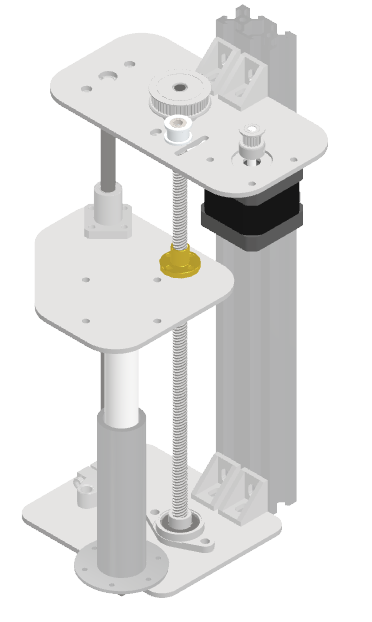
\includegraphics[scale=0.9]{figs/FinalExtruder.png}
    \caption{Final Syringe-Based Extruder Design}
    \label{fig:extruderFinal}
\end{figure}

This figure shows the refined version of Concept 3. It adds brackets to mount the platforms to the 2020 aluminium extrusion, includes a slot-and-idler-based belt tensioning mechanism, separates the syringe from the lower platform into two parts mounted together via the syringe’s flange. An E3D heater assembly is also mounted to the syringe's threaded nozzle in order to raise the temperature of the syringe.

\section{Gantry Design}
The design of a gantry enables the positioning of the extruder, allowing the system to function as a 3D printer. This section follows the same structure as the extruder design in which concepts are developed and evaluated, a single concept is selected and refined into a final design. 
\subsection{Concept Generation}
\subsubsection*{Concept 1}
The first concept (Figure~\ref{fig:Gantry1}) uses a CoreXY system with two steppers driving the XY belts and a third stepper that lifts the bed via a lead screw. The frame is made from aluminium extrusions, with linear rails guiding all horizontal motion. The Z-axis bed is guided by two shafts and bearings and the bed is comprises of a removable copper plate (to aid in manual process like curing or cleaning). 
\begin{figure}[H]
    \centering
    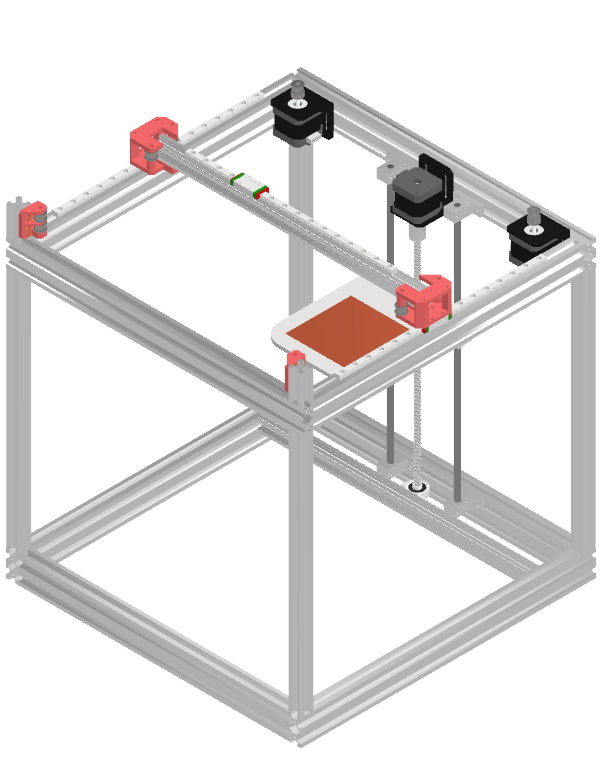
\includegraphics[scale=0.68]{figs/GantryConcept2.png}
    \caption{Concept 1 CoreXY Design}
    \label{fig:Gantry1}
\end{figure}

\subsubsection*{Concept 2}
In Figure~\ref{fig:Gantry2}, each axis is driven by its own lead screw(s) (all turned by NEMA 17 stepper motors), with wheel carriages guiding motion along aluminium extrusions. The bed is supported by two linear shafts with bearings and also has a removable copper plate. 
\begin{figure}[H]
    \centering
    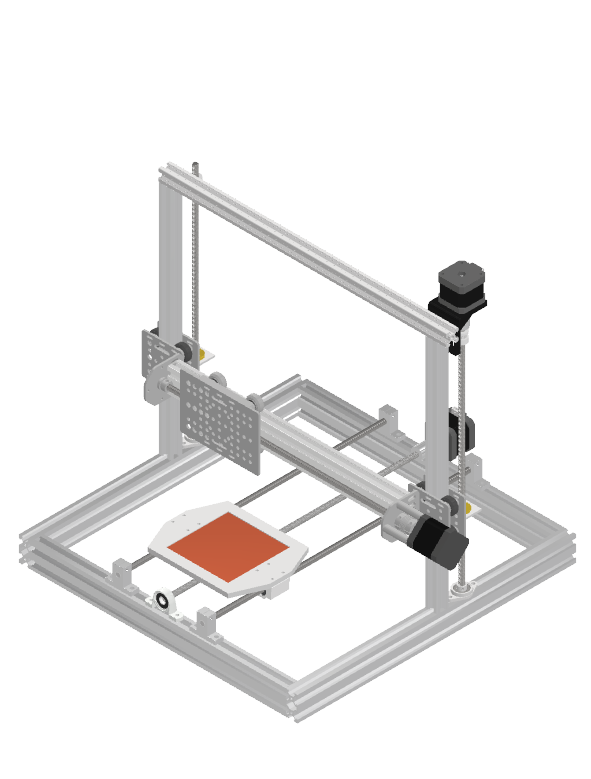
\includegraphics[scale=0.8]{figs/GantryConcept1.png}
    \caption{Concept 2 Bed-Slinger Design with only Lead Screws}
    \label{fig:Gantry2}
\end{figure}

\subsubsection*{Concept 3}
The final design, in Figure~\ref{fig:Gantry3}, uses two lead screws (synchronized by a GT2 belt), driven by one stepper, to lift the Z-axis beam. The extruder carriage is guided along the Y-axis v-slot aluminium beam and driven by a GT2 belt, while another belt drives the bed in the X-direction along two rods (like in Concept 2). The bed is a fixed aluminium plate to enable the addition of a permanent cooling mechanism (Peltier).
\begin{figure}[H]
    \centering
    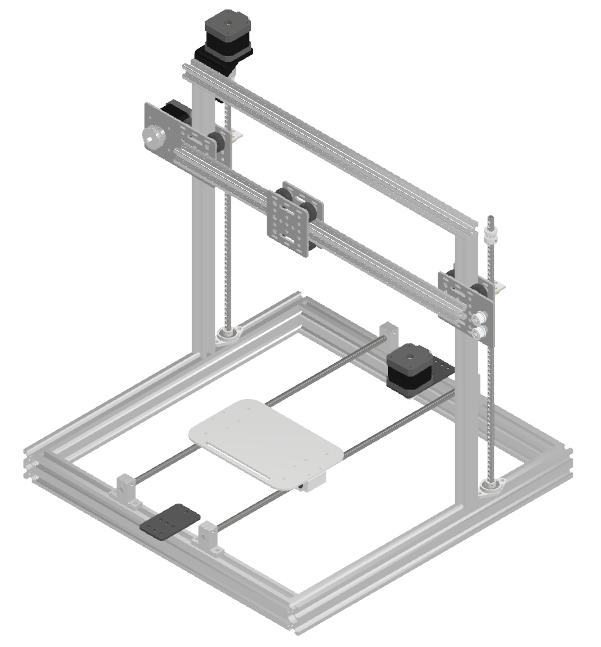
\includegraphics[scale=1]{figs/Gantry3.png}
    \caption{Concept 3 Bed-Slinger Design with Lead Screws and Belts}
    \label{fig:Gantry3}
\end{figure}

\subsection{Concept Evaluation and Selection}
The previously generated concepts are evaluated, as was done with the design of the extruder, with the purpose of selecting the concept that best satisfies the project’s stakeholder and engineering requirements. The evaluation is carried out in Table~\ref{tab:pugh2}, which compares each concept against a set of weighted criteria (based on the project's stakeholder requirements). These criteria include factors such as positional accuracy, speed, affordability, and sterilisability. Each factor was compared against Concept 2 (the datum) using a relative score of up to $\pm2$ (as with the extruder evaluation). The resulting scores were then totalled according to each criterion’s respective weight.
\begin{sidewaystable}[p]
\centering
\caption{Concept Evaluation (Pugh Chart)}
\label{tab:pugh2}
\renewcommand{\arraystretch}{1.2}
\setlength{\tabcolsep}{3.5pt}
\begin{tabular}{|>{\centering\arraybackslash}p{35mm}|
                >{\centering\arraybackslash}p{15mm}|
                >{\centering\arraybackslash}p{15mm}|
                >{\raggedright\arraybackslash}p{35mm}|
                >{\centering\arraybackslash}p{15mm}|
                >{\raggedright\arraybackslash}p{35mm}|
                >{\centering\arraybackslash}p{15mm}|
                >{\raggedright\arraybackslash}p{35mm}|}
\hline
\multicolumn{2}{|c|}{\textbf{Criterion}} &
\multicolumn{2}{c|}{\textbf{Concept 1}} &
\multicolumn{2}{c|}{\textbf{Concept 2}} &
\multicolumn{2}{c|}{\textbf{Concept 3}} \\
\hline
\textbf{Description} & \textbf{Weight} &
\textbf{Rating} & \textbf{Motivation} &
\textbf{Datum} & \textbf{Motivation} &
\textbf{Rating} & \textbf{Motivation} \\
\hline
% ---- Rows: duplicate as needed ----
Maximum XY speed (SR1) & 0.12 & +1 &  Uses belts & 0 & Limited by lead screw & +1  & Belts can achieve higher speeds \\\hline
XY positional accuracy (SR2) & 0.24 & -1 & Belts are less accurate & 0 & High accuracy of lead screws & -1 & Belts are less accurate \\\hline
Z positional (layer height) accuracy (SR2) & 0.24 & -1 & Uses lead screws but is susceptible to bending & 0 & Accurate due to lead screws & 0 & Accurate due to lead screws \\\hline
Sterilisability and cleanability (SR9) & 0.20 & 0 & Removable copper bed & 0 & Removable copper bed & -1 & Fixed bed \\\hline
Affordability (SR11) & 0.20 & -1 & Requires more parts (Idlers and tensioners) & 0 & Uses more expensive parts (lead screws compared to belts) & +2 & Simplest build with cost effective, standard parts \\\hline
% ---- Summary rows ----
\hline
\multicolumn{2}{|l|}{\textbf{Sum of plus ratings}} &
\multicolumn{2}{c|}{1} &
\multicolumn{2}{c|}{0} &
\multicolumn{2}{c|}{3} \\\hline

\multicolumn{2}{|l|}{\textbf{Sum of minus ratings}} &
\multicolumn{2}{c|}{-3} &
\multicolumn{2}{c|}{0} &
\multicolumn{2}{c|}{-2} \\\hline

\multicolumn{2}{|l|}{\textbf{Overall total}} &
\multicolumn{2}{c|}{-2} &
\multicolumn{2}{c|}{0} &
\multicolumn{2}{c|}{1} \\\hline

\multicolumn{2}{|l|}{\textbf{Weighted total}} &
\multicolumn{2}{c|}{-0.56} &
\multicolumn{2}{c|}{0} &
\multicolumn{2}{c|}{0.08} \\\hline

\end{tabular}
\end{sidewaystable}
\FloatBarrier

\noindent The results of Table~\ref{tab:pugh2}'s evaluation reveal that Concept 3 is the most suitable option of the three generated concepts, achieving the highest overall weighted score and therefore best satisfies the system's stakeholder requirements. While it is more difficult to clean/sterilise the bed after prints due to it being fixed to the linear bearings, it provides a base to mount a Peltier module for bed cooling which would not have been practical if the bed was removable. It also performs favourably in terms of speed and affordability, due to its use of standard GT2 belts that are often used in 3D printing. It can also achieve high layer height accuracy due to its use of synchronised lead screws. 

\subsection{Final Gantry Design}
Finally, Concept 3, needs to be refined and developed into a final gantry design that is ready for procurement and assembly.

\subsubsection*{Z Axis Stepper Requirements and Positional Accuracy}
To determine the stepper torque requirements, the mass driven by the synchronised lead screws must be approximated. This can be done using Inventor Professional’s iProperties feature, which revealed that the total volume of the portion of the final design (extruder, horizontal beam, motors, and carriages) being lifted in the Z-direction is \SI{688658.130}{\milli\meter^3}. By assuming the average density of this assembly is \SI{2.7e-6}{\kilogram\per\milli\meter^{3}} (the density of aluminium), the mass to be moved by the lead screws is approximated as \SI{1.86}{\kilogram}. 

Appendix A.2, using the same lead screw properties as A.1, shows that this requires a minimum stepper torque of \SI{0.0388}{\newton\meter}. The final design uses a Creality 42-40 Stepper Motor that is capable of a holding torque of up to \SI{0.4}{\newton\meter}. The lead screw torque therefore has a safety factor of roughly 10 to allow for the system to achieve high accelerations along the Z-axis.

Finally, the positional accuracy of the Z-control must be characterised. The chosen stepper has a step angle of $1.8^\circ$ and the TR8x8 lead screws have a lead of \SI{8}{mm}. Therefore the positional resolution is:
\begin{align*}
\Delta z_{\text{Full Step}} &= \text{Lead} \times \frac{\theta_{\text{Full Step}}}{360^{\circ}} \\
&=8.00\times \frac{1.8^\circ}{360^\circ} \\
&= 0.04~\text{mm}/\text{step}
\end{align*}

\noindent This theoretical accuracy exceeds the \SI{50}{\micro\meter} requirement established in PR3. It should be noted that an even higher resolution can be achieved with microstepping.

\subsubsection*{X and Y Axis Stepper Requirements and Positional Accuracy}
Autodesk Inventor Professional can be used to reveal the final extruder has a total volume of \SI{379353.531}{\milli\meter^3} and the printer bed with its linear bearings, heat sink, Peltier and cold plate (shown in the final design later in Figure~\ref{fig:gantryFinal}) has a total volume of \SI{145105.084}{\milli\meter^3}. As done previously, by multiplying these volumes by the density of aluminium (\SI{2.7e-6}{\kilogram\per\milli\meter^{3}}), yielding two separate mass approximations of \( m_x = 0.39\,\text{kg} \) and \( m_y = 1.02\,\text{kg}\). By further assuming the carriages' friction coefficient to be 0.2 and the maximum horizontal acceleration to be \( a = 5\,\text{m/s}^2 \), the required stepper torque can be determined for each axis, as shown in Appendix A.3. The X-axis uses a GT2 pulley with 20 teeth and the calculations show that the stepper requires $0.0173\,\text{Nm}$ of torque and the Y-axis stepper (which uses a 36 teeth pulley) needs $0.08137\,\text{Nm}$. Therefore, the chosen NEMA 17 steppers have a holding torque up to \SI{0.28}{\newton\meter} for the X-axis and \SI{0.4}{\newton\meter} for the Y-axis.

With these described specifications, the positional accuracy in horizontal plane can be determined. Considering the use of pulleys in both the X and Y directions, the resolution can determined by multiplying the motors step angle with the radius of each pulley ($r_x=6.365$ and $r_y=11.46$):
\begin{align*}
    \Delta x &= \theta_{\text{Full Step}}\times r_x=1.8^\circ\frac{\pi}{180^\circ}\times6.365=0.200\,\text{mm}\\
    \Delta y &=\theta_{\text{Full Step}}\times r_y=1.8^\circ\frac{\pi}{180^\circ}\times11.46=0.360\,\text{mm}
\end{align*}
These fall short of the target set in PR2, but both fall within the acceptable range. However, they can be configured to meet the target by using the drivers to enable microstepping of at least 1/4.
\subsubsection*{Final Gantry}

\begin{figure}[H]
    \centering
    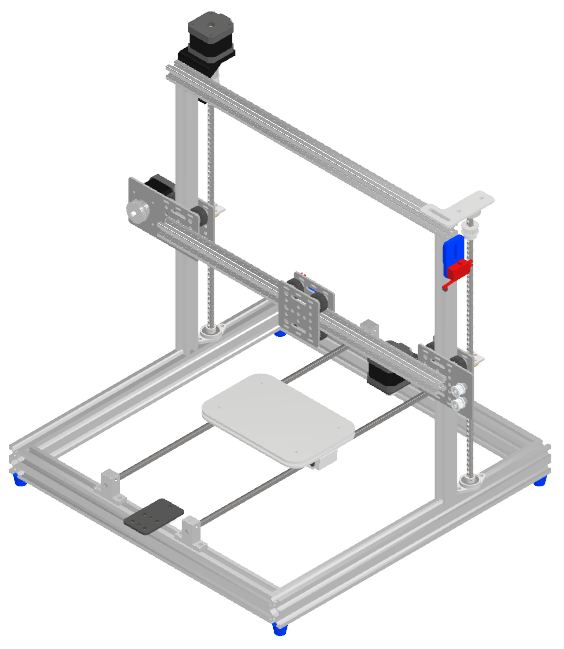
\includegraphics[scale=0.8]{figs/FinalGantry.png}
    \caption{Final Bed-Slinger Gantry Design}
    \label{fig:gantryFinal}
\end{figure}
The final gantry design is shown above in Figure~\ref{fig:gantryFinal}. It is the refined design, based on Concept 3, and incorporates a Peltier cooler mounted to the bed between two plates (cold side on top and heat sink at the bottom). The figure also shows the system's limit switches for homing.
\section{Final Design}
\noindent
The complete bioprinter design, shown in Figure~\ref{fig:bioprinterCAD}, shows the extruder and gantry subsystems, integrated into a single mechanical system. The extruder is designed to use a custom syringe, heater block, and load cell to deposit viscous gels at a controlled flow rate and temperature, while the gantry accurately positions it in 3D space to enable it to print three dimensional scaffolds. This final design concludes the mechanical design of the project and forms the basis for the embedded systems design and integration to enable the printer to function as required and undergo experimental validation.

\begin{figure}[H]
    \centering
    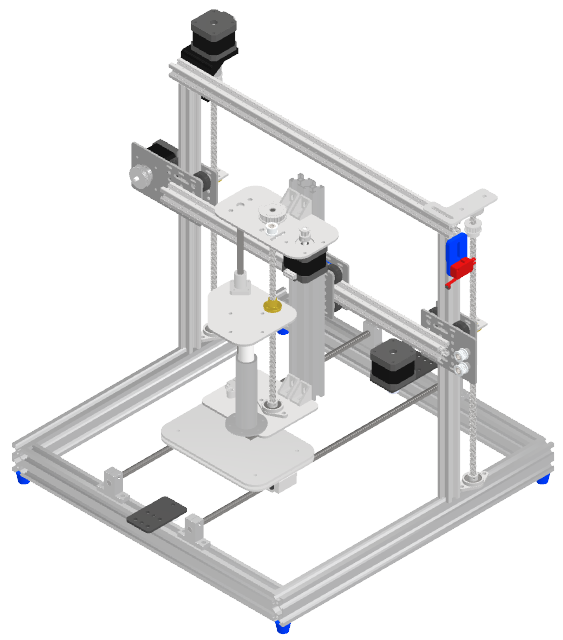
\includegraphics[scale=1]{figs/FinalBioprinter.png}
    \caption{Final Bioprinter Design}
    \label{fig:bioprinterCAD}
\end{figure}